\section{The Data Acquisition Toolkit}

%%%  An introduction of the idea of the "DAQ toolkit"
%%   mention Gen-I, Gen-II, Gen-III somewhere

%The New ROD Complex (NRC) is designed as a plug compatible replacement for the current complex. The interfaces necessary to satisfy that plug compatibility were described in Chapter 1. At one level of abstraction the physical implementation of the NRC could be simply represented as an arbitrary aggregate of PCB boards. But, of course, because these boards operate to a single purpose, they will also necessarily require connections between them. Typically, for reasons of understanding, modularity and maintenance, those connections follow predefined, accepted mechanical and electrical standards. In this document any such usage which employs a specific standard will be referenced as a Platform. For example, VME would constitute one such platform. For the NRC that platform is based on an existing standard developed by the PCI Industrial Computer Manufactures Group (PICMG) commonly referred to as the Advanced Tele-Communication Architecture, or ATCA, whose current revision is referred to within that consortium as PICMG 3.0. As a platform ATCA is now quite mature, having been in existence for more than ten years, with a broad design base and a wealth of equipment deployed in the field as well as a burgeoning eco-structure within the telecommunication and defence industries.
%ATCA usage by the NRC will be entirely compliant with the PICMG 3.0 specification. That specification is described in [6] with an introduction available from [5]. However, the remainder of this section is intended to provide sufficient background to gain a thorough understanding of the physical design description.



\subsection{Advanced Tele-Communication Architecture and the ATCA Shelf}
\label{sec:ATCA}

The ATCA shelf is known historically as the chassis and is by analogy, equivalent to a VME crate. Shelves house the Front-Boards and RTMs described below (see Sections \ref{sec:frontboard} and \ref{sec:rtm}). They contain, from front to rear, pairs of slots with each pair housing a Front-Board in the front and the Front-Board's corresponding RTM in the rear. The shelf allows for hot-swap of any board in any slot. Depending on form factor the number of its slot pairs varies from two (2) to sixteen(16). The orientation of those slots also varies, as shelves are offered with either horizontal or vertical orientation. In turn, that orientation affects the flow of air; from either left to right (horizontal), or top to bottom (vertical).
Broadly, the shelf is composed of a sub-rack, backplane, filters and cooling devices (fans). The subrack provides the infrastructure to contain the Front-Boards and RTMs described below. This includes guide rails, ESD discharge, alignment, keying, and backplane interface. Backplanes are passive circuit boards which carry the connections between slots. Although somewhat more complicated in detail, for this document, those connections can be partitioned into three logical groups: power, control and differential data pairs. The topology for both power and control connections is invariant of backplane. However, in order to accommodate different applications the connection topology of data pairs can vary. Two commonly used topologies are the dual star and full mesh.The backplane (and ATCA) is protocol agnostic with respect to the usage of these differential pairs with the choice delegated to the shelf's specific Front-Boards.

\begin{figure}[tbh]
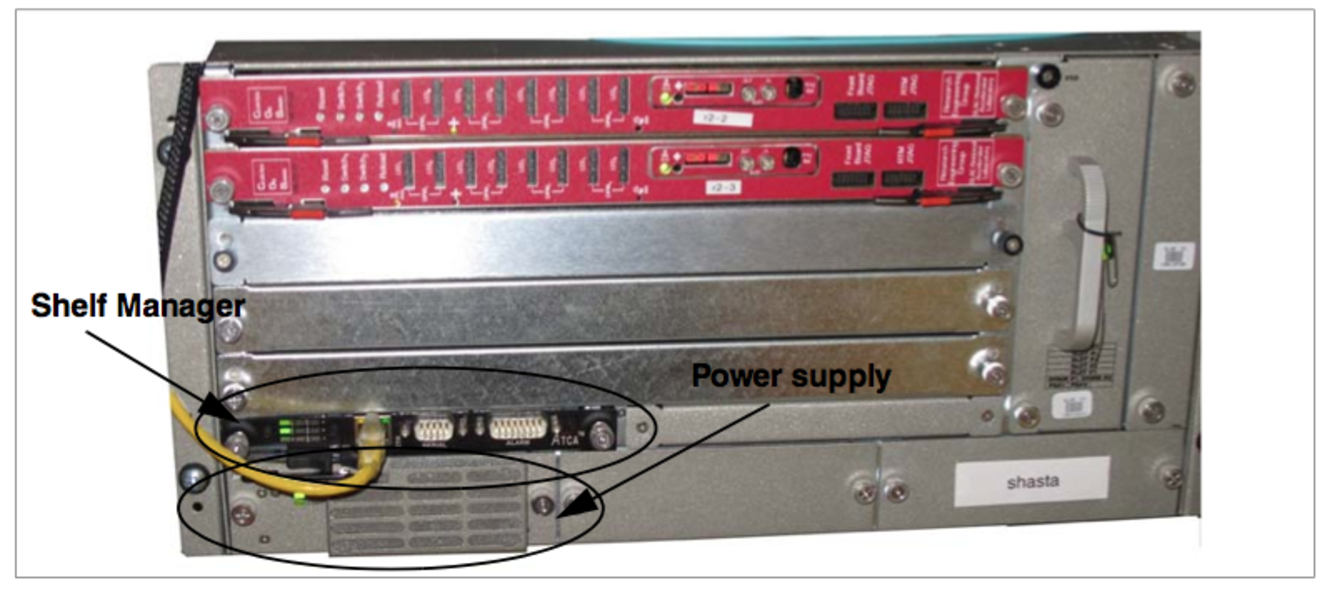
\includegraphics[scale=0.8]{shelf-front.pdf}
\caption{Front view of 5-slot ATCA shelf.}
\label{fig:frontShelf}
\end{figure} 


This photograph is of a COTS1 shelf purchased from ASIS [7]. It has a horizontal orientation within its corresponding rack with airflow from left to right. It contains a replicated, full mesh backplane. Two of its five front slots are populated with Front-Boards, while its unused slots are populated with dummy air baffles. Note the RJ45 connector located on the front-panel of its Shelf-Manager (ShMC). This provides the shelf manager access to the Ethernet from which control and monitoring (through IPMI) of the shelf would be accomplished. Further, note the integral power supplies. These supplies are not required by the ATCA standard, but are provided by ASIS as a convenient feature for bench-top usage. The same shelf viewed from the rear is illustrated in Figure \ref{fig:backShelf}.

\begin{figure}[tbh]
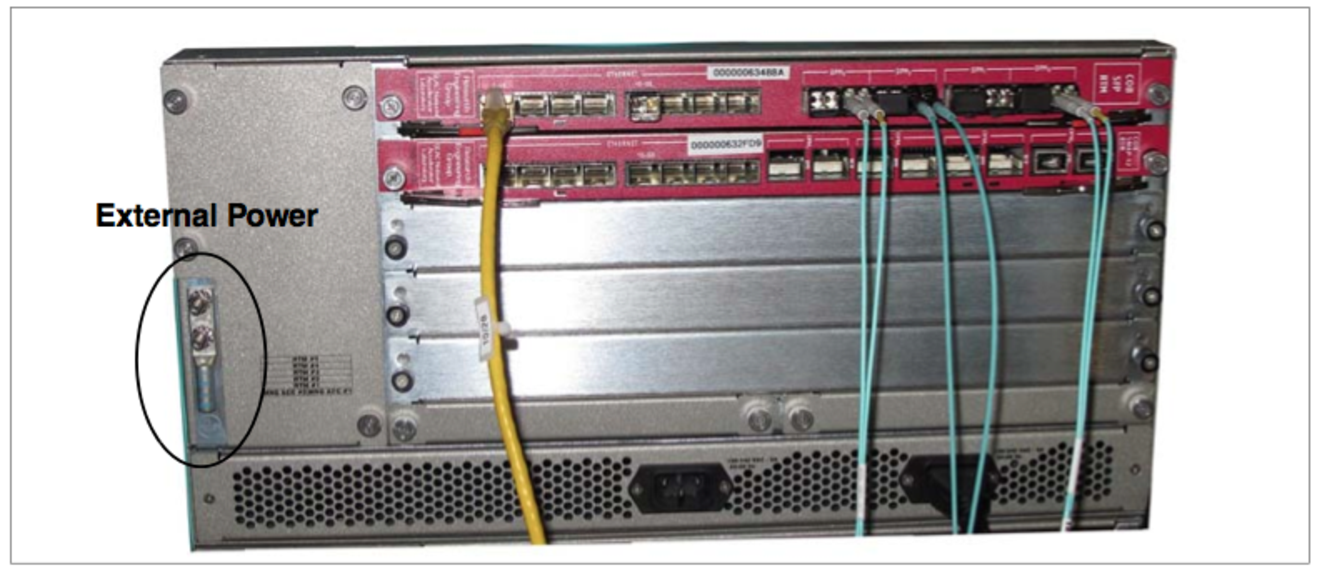
\includegraphics[scale=0.8]{shelf-back.pdf}
\caption{Back view of 5-slot ATCA shelf.}
\label{fig:backShelf}
\end{figure} 


\subsubsection{The Front-board}
\label{sec:frontboard}
The Front-Board constitutes the heart of the ATCA eco-system. From a shelf's perspective that board is simply a PCB board, 8U wide x 280 mm deep and which plugs into one of its front slots. That board, although following ATCA mechanical and electrical interface standards, contains logic which is application specific.  The board's rear side contains three logical “Zones”. Zones 1 and 2 connect directly to a shelf's backplane. Zone 1 provides access to shelf power (+48 VDC) as well as the I2C communication channels which the board uses to communicate with its shelf manager. Zone 2 provides access to the high-speed, differential pairs connecting boards together. The area encompassed by Zone 3 is application defined, but reserved for connections to the board's RTM.
LBNE requires one application specific Front-Board. That board is described in Section \ref{sec:COB}.
A photograph of a representative Front-Board, showing connectivity to an RTM (using PICMG 3.8) is illustrated in Figure \ref{fig:frontBoard}.

\begin{figure}[tbh]
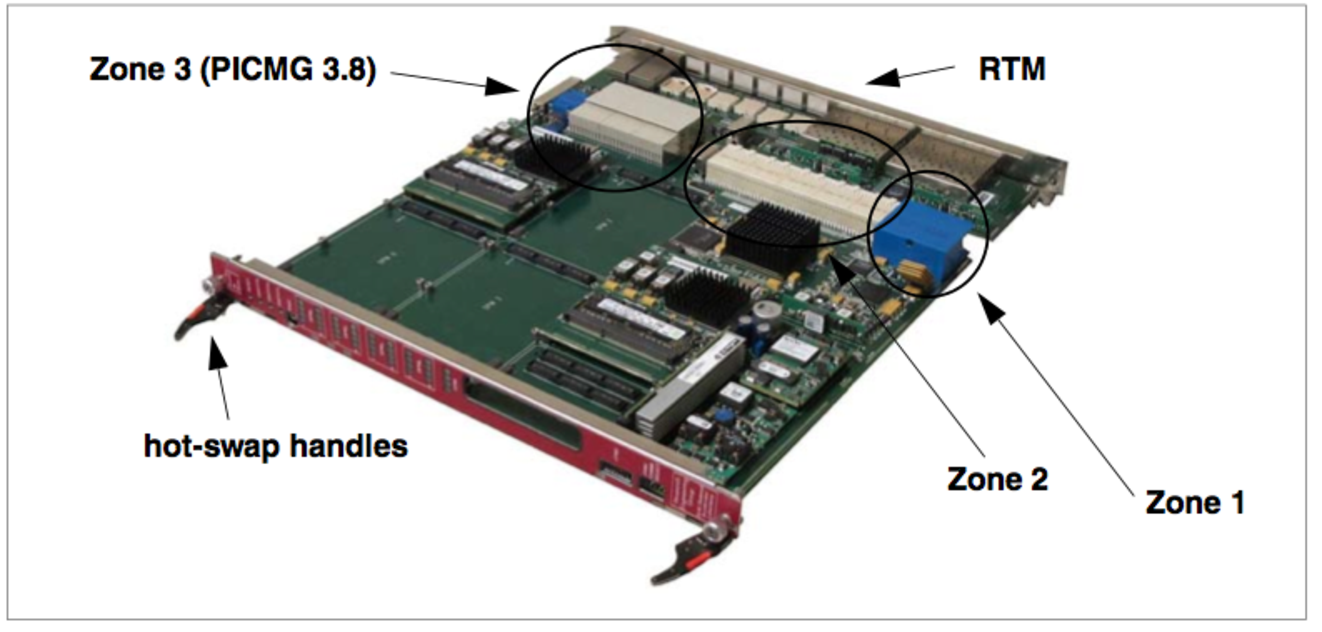
\includegraphics[scale=0.8]{front-boardpdf.pdf}
\caption{Representative ATCA front-board.}
\label{fig:frontBoard}
\end{figure} 

\subsubsection{Rear Transition Module}
\label{sec:rtm}
The RTM (Rear-Transition-Module) is simply a PCB board, 8U wide x 70 mm deep which is used to extend a Front-Board and  house a board's external, I/O interface. The RTM shares the same hot-swap model as the Front-Board and specifies an identical pitch (1.2"). This allows the RTM to reuse the same panel, handle switches, and LEDs as its Front-board. The RTM connects to its Front-board through Zone 3. The form of that connection is application specific. However, if power for the RTM is necessary, it must be provided by the Front-board and must be brought through Zone 3. The ATCA specification is somewhat ambiguous with respect to the maximum power drawn by an RTM.   Zone 3 is populated with two connectors, one for power and one for signal. Power provided through the power connector is +12 VDC and that connector also contains pins for JTAG as well as I2C support. The I2C channel is expected to be used by the Front-Board for control of the RTM's hot-swap switch as well as its front panel LEDs.
The signal connector provides up to 120 differential pairs. How those pairs are assigned between Front-Board and RTM is considered application specific. However, for LBNE's Front-Board, each one of its four DPM bays is assigned 1/4 of those pins or thirty (30) pairs (see Section \ref{sec:COB}).

%\subsubsection{IPMI and Shelf Manager}
%\label{sec:shelfManager}
%ATCA adapts a somewhat locally autonomous philosophy with respect to environmental control and monitoring. As part of this model, each shelf has associated with it a single entity responsible for maintaining the health and safety of its infrastructure. That entity is called the Shelf Manager (ShMC). Front-Boards, through their own local controller (or IPMC) negotiate both individually and independently with their shelf manager for their own activation or deactivation. They do so by publishing changes to their state through dedicated I2C channels on the backplane.
%The shelf manager determines, based on hot-swap interface, when a board requires activation or deactivation. Power levels are negotiated based on both a board's request and the shelf's total available power. Shelf temperatures are maintained at safe levels autonomously by the shelf manager using information published by each board and adjusting power levels and fan-speeds accordingly.
%In short, once a shelf's power is applied and while its shelf manager is active, no external monitoring or control is necessary to maintain the shelf's health and safety.
%Although the health and safety of its shelf is maintained autonomously, the shelf manager still has provision for an external interface. Through this interface any information published to the shelf manager can be exported and the shelf manager can itself be configured. That physical interface is Ethernet and the shelf manager contains a TCP/IP Stack through which external communication is maintained. The logical interface for control and monitoring of the shelf is IPMI [18] and a wealth of tools exist, which interact with this interface.


\subsection{Cluster-on-Board}
\label{sec:COB}
The COB (Cluster-On-Board) is an 8U, ATCA compliant Front-Board with a PICMG 3.8 Zone 3. Functionally, the COB serves as a carrier board for the RCEs hosting the firmware and software developed for LBNE (see Section \ref{sec:RCE}). Those RCEs are mounted on mezzanine boards (see Section \ref{sec:Mezzanine}), which in turn plug into Bays on the COB. Bays are connected to the COB's two separate, independent Interconnects as well as its Zone 3 connectors. Interconnects provide arbitrary, high speed communication paths between the elements contained on the bay's mezzanine boards, both (it is important to note), inter and intra COB.
Although rated up to 300 watts, when fully populated with five mezzanine boards, a COB draws closer to 120 watts. This board is one deliverable from SLAC's R \& D program on high-speed DAQ. As such, LBNE simply purchases this board and from its perspective, that board consequently requires neither design nor development. A photograph of that COB (in preproduction form) with its five bays occupied is shown in Figure \ref{fig:cob}.


\begin{figure}[tbh]
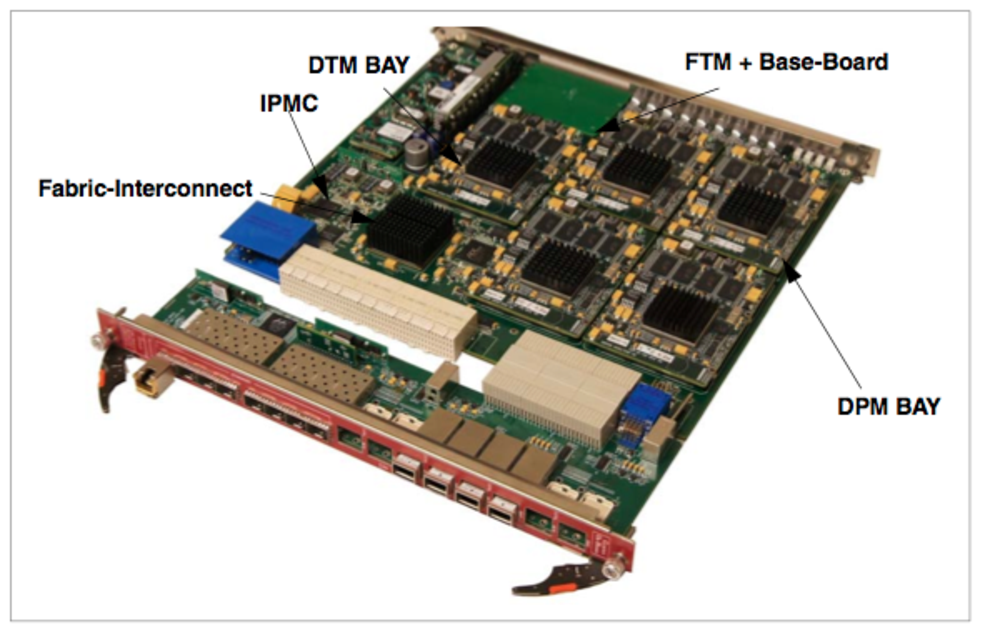
\includegraphics[scale=0.8]{cob-photo.pdf}
\caption{Pre-production COB.  }
\label{fig:cob}
\end{figure} 


The COB contains five (5) bays; one (1) DTM bay and four (4) DPM bays. Although all bays share identical form factors and connectors, they can be differentiated, primarily by how they connect to Zone 3, with the DTM connecting only to its power connector and the DPM only to its signal connectors. In turn, those connections determine the function of their corresponding mezzanine boards. The DTM, interacting with its shelf manager, manages the health and safety of both COB and RTM, while DPMs acquire and process data originating from the RTM. Those data, their interface, acquisition and processing are all intended to be application specific.
%subsubsection{The DTM Bay}

The mezzanine board plugged into the DTM (Data-Transport-Module) bay contains one RCE as well as the COB's IPM Controller (IPMC). The IPMC is the element responsible for monitoring the underlying health and safety of the COB as well as its corresponding RTM. It is also responsible, in conjunction with its corresponding shelf manager, for board and RTM activation/deactivation. It performs all these activities by interacting with various components on the COB, specifically with the RCEs contained within the COB's five bays. That interaction is accomplished through dedicated, local I2C busses. The IPMC is a SOC (System-On-Chip), containing a dedicated ARM based (M3) processor. That processor runs de-facto, industry standard Pigeon-Point IPMC firmware and software [41], suitably modified to control and monitor the specific functionality of the COB.


Although in capability and form no different than any other RCE, the DTM's RCE has the fixed, dedicated responsibility for managing both of the board's interconnects. For this purpose it contains specific firmware and software. For example, as one responsibility, it must maintain the configuration and supervise the 10G-Ethernet switch contained within the fabric interconnect. That switch's management interface is a single lane PCIe. To communicate with this switch, the RCE contains a PCIe Protocol-Plug-In (firmware, see Section \ref{sec:RCE}) as well as the tools (software) to configure and monitor that switch. Note, however, that while the DCM's RCE has predefined, base responsibilities it also remains accessible for user applications.
%subsubsection{The DPM Bay}

The mezzanine board plugged into a DPM (Data-Processing-Module) bay contains two (2) RCEs. Each DPM provides connections to thirty (30) differential pairs originating from the RTM, but carried through the COB's Zone 3 signal connector. The mapping of those thirty pairs to the mezzanine board's two RCEs is arbitrary and determined by application. The function of either RCE is determined not only by the mapping of those thirty pairs, but by the firmware and software it contains.
%For LBNE, that function will be either as a Feature Extractor or as a Formatter (see Section 2.2).

\subsection{Interconnects}
\label{sec:Interconnects}
The fabric interconnect contains, as its principal feature, a local, 10-Gigabit Ethernet (10-GE). Packets are switched on that network using a commercial  ASIC. That ASIC is a fully compliant Layer-2, 10G-Ethernet switch. Although fully provisioned for buffered transfer, switch operation is, by default, cut-through with an ingress/egress latency of less than 200 Nanoseconds. It is also a fully managed switch with a PCIe interface connected to the DTM's RCE. Through its interconnect the COB's RCEs appear as nodes on that Ethernet. The interconnect allows its physical network to be extended to both nodes and networks external to the COB. Those networks could be, for example, other COBs residing in the same shelf, or even nodes physically disjoint from both COB and its shelf.
%
%Internal to its shelf, the interconnect extends its network through its connections to Zone 2 of its backplane, specifically those connections to that backplane's fabric interface. The interconnect has individual connections to each of the thirteen slots of the shelf's backplane. With a full mesh backplane, this allows each network of every COB to be connected to each network of every other COB. External to its shelf the interconnect extends its network through its connections to the COB's fiber-optic transceiver bay. That bay can contain up to eight (8) SFP+ transceivers [20].
%The interconnect's switch is organized in units of Ports. Each port is composed of four lanes and each lane is constructed from two differential pairs. Each lane forms a full-duplex channel with one pair allocated for transmission and one pair for reception. Each lane of each port is capable of operating independently at a fixed set of speeds ranging from 1.0 Gigabits/second up to 12.5 Gigabits/second. Lanes may also be bound together to form a single Ethernet channel which operates at four times the speed of any one lane. For LBNE, which carries 10-GE, the switch is configured to run XAUI, requiring four lanes, each operating at 3.125 Gigabits/second. The switch contains twenty-four (24) ports. Those twenty-four ports are allocated to the fabric interconnect as follows:
%\begin{itemize}
%\item One (1) port connected to the DTM bay (one RCE).
%\item Eight (8) ports connected to the four DPM bays (two per bay, one for each RCE).
%\item Two (2) ports are connected to the SFP+ transceiver cage.
%\item Thirteen (13) ports are connected to the fabric interface (P2).
%\end{itemize}
%In short, within a shelf, the fabric interconnect allows for the formation of a uniform Ethernet populated with a flat space of RCE nodes.

The base interconnect's principal function is to manage and distribute synchronous timing to the COB's five bays. Note that unlike the fabric interconnect the protocol distributed over this interconnect is application specific. In further contrast to the fabric interconnect which functions identically independent of the shelf slot it occupies, the base interconnect has slot dependent responsibilities. This is a consequence of the fact that while the fabric interconnect uses ATCA's fabric interface, the base interconnect uses its base interface. That interface employs a backplane topology that is fixed by the standard at dual-star. ATCA refers to slots at its roots as Hub slots and slots at its leaves as Node slots. Necessarily, the behavior of a board, specifically its base interconnect, must vary depending on whether it occupies either a hub or a node slot. While boards in node slots need only distribute timing locally, boards occupying node slots must distribute timing not only locally, but also to other boards occupying its shelf. In short, while occupying a hub slot the base interconnect drives its base interface, but while occupying a node slot receives timing.
%%%%%%  this part I need to check with Ryan & Mike...
%The distribution model for the base interconnect allows timing to originate from one of three potential sources:
%\begin{itemize}
%\item Internal, where the source is the base interface.
%\item External, where the source is the COB's Front-Transition-Module (FTM).
%\item Local, where the source is the COB's DTM.
%\end{itemize}
%Internal timing was described above. External timing allows the timing source to originate off the shelf. The FTM is a bay which contains an application %specific, small “PMC-like” daughter board. Logically, the FTM serves the same role on the front of the COB as the RTM does on its rear, that of media %adaptation. Eight (8) differential pairs from this daughter board connect directly to the base interconnect and eight (8) differential pairs connect to the %DTM's RCE. Those eight pairs are intended to allow that RCE supervision of the FTM. Local timing allows the board to operate either stand-alone or %perhaps more usefully provide a simulation of timing which would normally be sourced either internally or externally.
%LBNE has purpose built versions of both FTM and base board. Those version are described in Sections 2.6.5 and 2.6.6:


\subsection{Reconfigurable Cluster Element}
\label{sec:RCE}
The RCE (Reconfigurable-Cluster-Element) is a bundled set of hardware, firmware and software components. Together, those components form a generic computational element targeted to process efficiently, with low latency, those kinds of data found passing through HEP DAQ systems. Those data have in common three features which make specific, somewhat, competing demands on the functionality of any such element. Those features are:
\begin{itemize}
\item Highly parallel: Data which are massively parallel are most naturally also processed in parallel, requiring computational elements which scale in cost,   footprint and power. Those elements, in order to manage the flow of their data both efficiently and coherently, communicate together. This necessitates a communication mesh which shares the same scaling properties as the elements themselves.
\item Inhomogeneous: As those data typically originate with their corresponding detector they are carried necessarily over a variety of media employing various inhomogeneous protocols. The element's I/O structure, must support, naturally, without sacrifice of performance that diversity.
\item Transient:
Transient data arrive at an element once, to be either transformed or reduced before immediately exiting the element. Such data are not typically amenable to caching strategies and require elements whose optimal computational model emphasizes a performanent efficient I/O structure, coupled strongly to a large, low latency memory system over raw processor speed.
\end{itemize}
The RCE is optimized for those three features. Physically, one element can be contained in a footprint of less than 32 cm$^2$, typically draws less than eight (8) watts, costs (in small quantities) around \$750 and contains a native 10-Gigabit Ethernet interface. Elements are connected through a commercial, commodity ASIC containing a 64 channel, Layer-2, cut-through1, Ethernet switch [38]. The combination of elements and switch define a Cluster and the nature of ethernet as well as functionality within that switch allows for the composition of arbitrary numbers of cluster hierarchies. For example, from the RCE perspective, the COB represents a single cluster of nine (9) RCEs and its ATCA shelf is simply a container for a single level hierarchy of up to fourteen (14) nine node clusters. A block diagram of the major physical features of the RCE is illustrated in Figure \ref{fig:RCEblock}.


\begin{figure}[tbh]
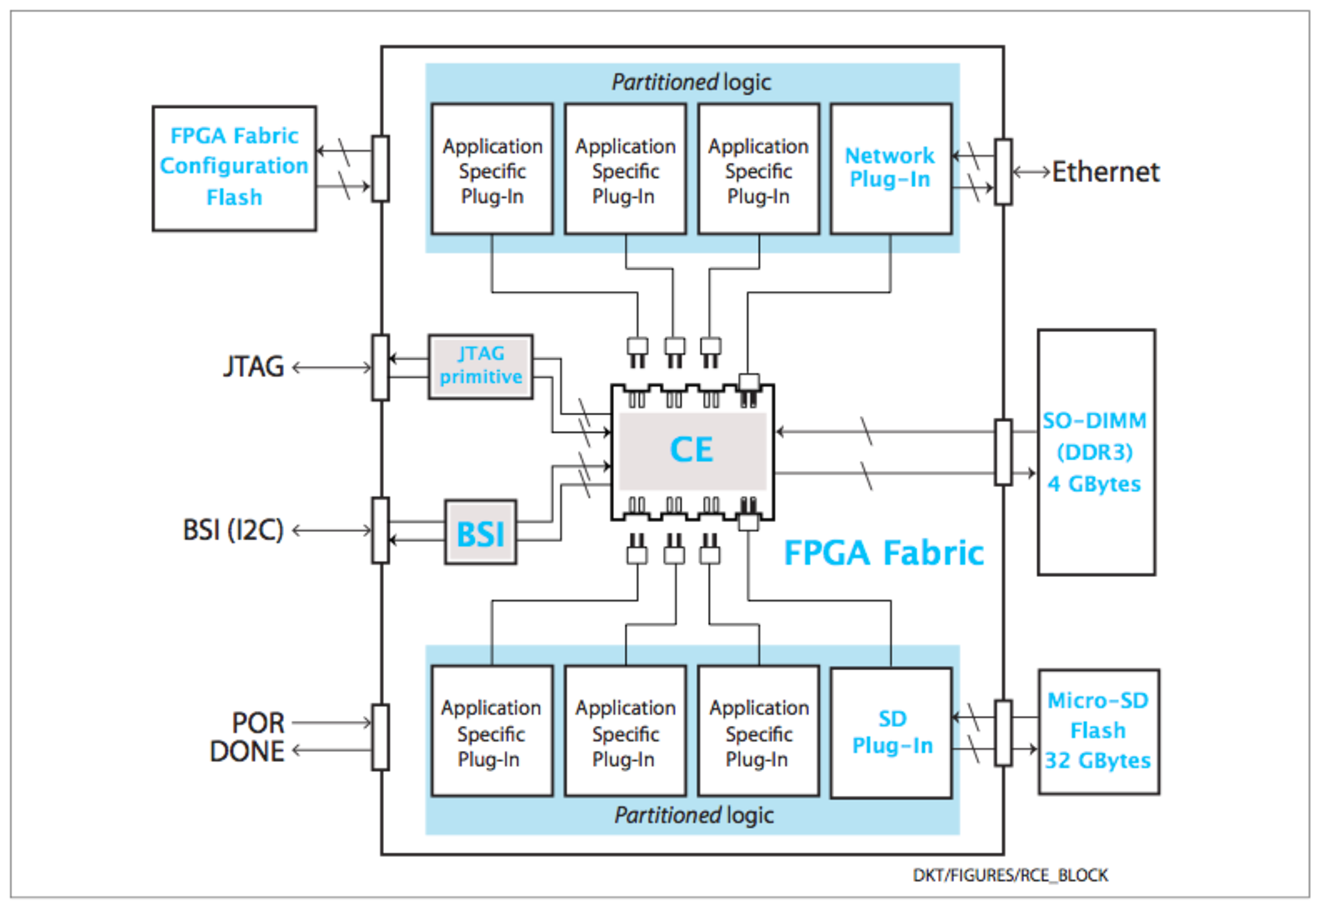
\includegraphics[scale=0.8]{rce-block.pdf}
\caption{Block diagram of the RCE.}
\label{fig:RCEblock}
\end{figure} 

The principal implementation feature of the RCE is in its reuse of System-On-Chip (SOC) technology, specifically, member's of Xilinx Virtex-5 FX family [55]1. As such, the RCE is neither processor, FPGA or DSP. Instead, it can be simultaneously any combination of the three. Within its fabric the FPGA contains both soft (user defined) and hardened (manufacture defined) silicon. That fabric is configured automatically on POR (Power-On-Reset) and is either downloaded directly from images previously stored on the FPGA's configuration (platform) flash, or indirectly through the RCE's JTAG interface. Note also that the platform flash is itself programmed through the RCE's JTAG interface. The RCE employs standard Xilinx tools and software to program the FPGA.
Xilinx refers generically to its set of different, hardened silicon as resources. Among the more important of those resources are high speed serializers/deserializers, I/O adapters, DSP tiles, dual-port RAM and of course, its processor. The RCE allocates the processor as well as a modest number of additional resources and soft silicon for its CE (Cluster-Element). The CE has exclusive use of, but interfaces indirectly with its external DDR3 memory and micro-SD flash system. Memory is packaged as SO-DIMM and the micro-SD flash is removable, allowing its capacity to be determined by user application.

The BSI‘s (Boot-Strap-Interface) principal function is to reset the CE. However, it also contains the initial configuration information necessary for the CE's bootstrap loader to boot its processor. The BSI is outside the CE so that its configuration may be retained over resets of the CE. External to the FPGA the BSI appears as a standard I2C device and receives its command and control through that interface. Note, for the COB, that device is controlled and monitored through its IPMC.

To provide isolation between system and user firmware and insure reproducible behavior, system firmware is partitioned [53] away from application specific logic. System firmware is defined as the CE, the BSI, JTAG support and both Network and SD Plug-Ins.
The CE, which is both at the heart of the entire RCE and contains a significant fraction of the user's intellectual investment is described in Section \ref{sec:CE}. The remainder of the fabric, both hardened and soft silicon is reserved for application specific logic. That logic and its relationship with the CE is described below.

Although both user defined and implemented, any application specific logic, does of course require information exchange between it and its CE1. The interface model which allows such exchanges is the plug and socket. To follow that model, the user wraps their implementation specific logic with a thin veneer of system provided firmware. That wrapper is the plug and the combination of user logic and its plug is called a Protocol-Plug-In or PPI. When wrapped, that logic is now capable of being plugged into any of the eight predefined sockets on the CE. And once plugged in, both PPI and CE are now able to exchange information.

Although bundled with its base system the RCE itself takes advantage of this model to “glue” its Ethernet and SD interfaces to the CE. Both are good examples of one class of PPIs which must interface outside their FPGA.  Such PPIs when plugged into their CE have as their closest analogy the classic I/O device and processor model. However, unlike that model the PPI model coupled with the resources offered by the FPGA fabric provides an essentially unlimited way to either customize or mold the CE to arbitrary devices and protocols. Of course, the user is not limited to using the fabric and its resources solely for I/O. One can define PPI whose sole purpose is to take advantage of the DSP tiles and combinatoric logic of the FPGA to process rather than transfer data. LBNE can use this functionality to its advantage in performing its feature extraction.

\subsection{The Cluster Element}
\label{sec:CE}
The essential function of the CE is as a platform which serves as an application specific nexus for the data both received and transmitted through the RCE's application specific PPIs. As such, the CE can be considered as both a hardware1 and software platform. As a hardware platform its principal blocks are illustrated in Figure \ref{fig:CEblock}. As a software platform its corresponding services are described in Section \ref{sec:Services}.


\begin{figure}[tbh]
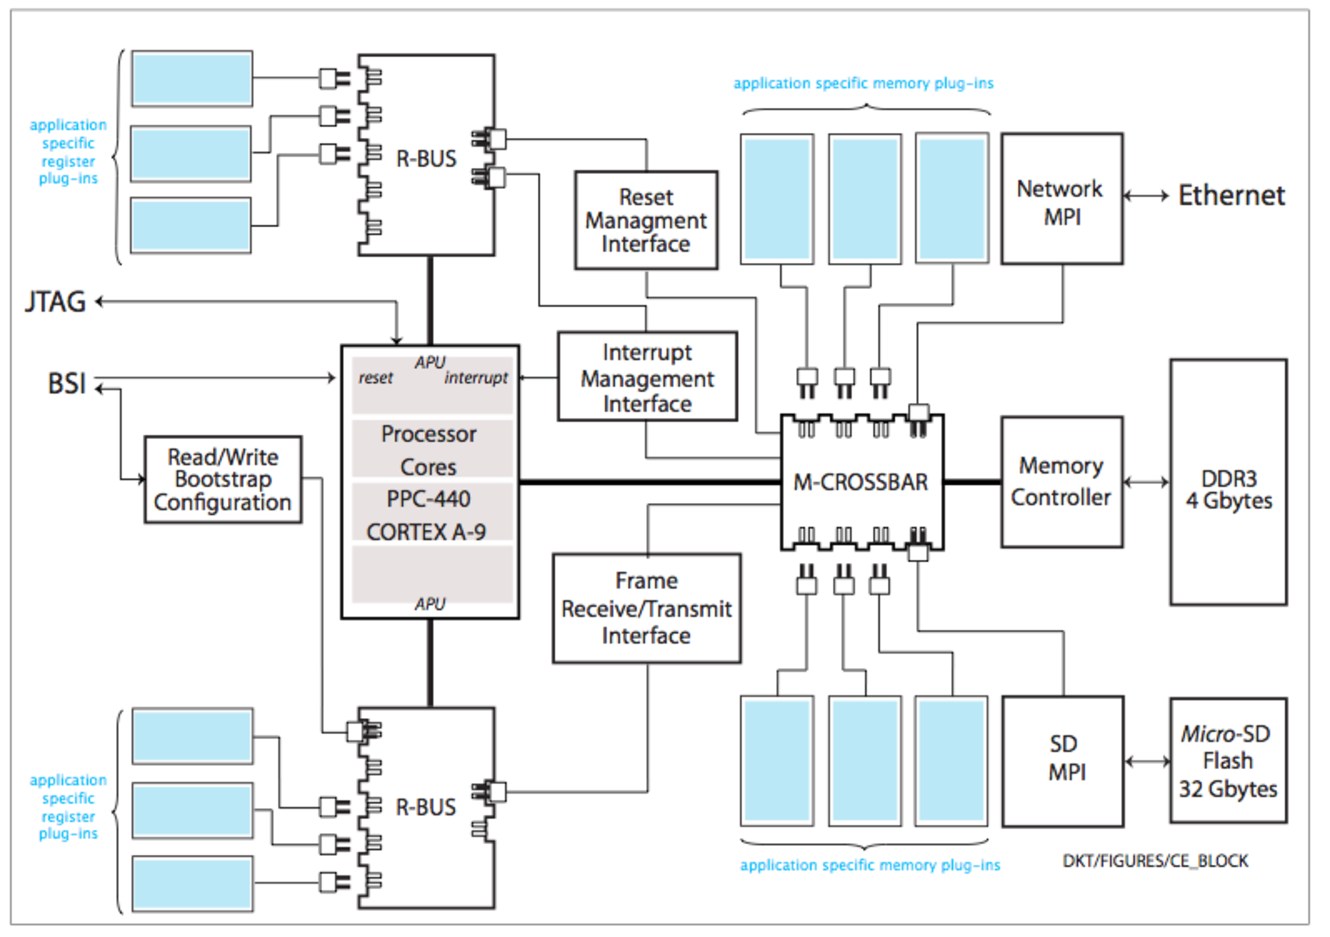
\includegraphics[scale=0.8]{ce-block.pdf}
\caption{Block diagram of the CE.}
\label{fig:CEblock}
\end{figure} 


Its principal implementation blocks are its Memory Controller, Crossbar and Processor:
The Memory Controller: Interfaces the RCE's external memory with the CE's Crossbar. It is a soft controller, derived from an existing Xilinx DDR2 design, but tailored for usage of low latency, DDR3 memory. The controller allows addressing of up to four (4) Gbytes of memory. It is clocked at 320 MHZ, has separate, internal, 64-bit, read and write datapaths providing roughly 5 Gbytes/second of either read or write bandwidth.
\begin{itemize}
\item The Crossbar: The Crossbar interconnects memory controller, processor1, and up to eight (8) PPI sockets allowing for autonomous, concurrent transfers between all three types of entities and providing arbitration for when those transfers might collide. The crossbar is clocked at the same rate as its memory controller (320 MHZ) and contains internal, separate, 128-bit, read and write datapaths. Its core is hardened silicon [56], but suitable enhanced with purpose built firmware which glues the eight PPI sockets to that core.
\item The Processor: A 32-bit, PowerPC-440, superscaler, single core, RISC processor with separate 32 Kbyte data and instruction caches [56]. It is clocked at 475 MHZ. In addition to the three busses connected to the crossbar, the processor contains another, separate, independent, 128-bit wide bus called its APU bus [56]. One side is connected to the processor and its other side is an interface to the FPGA‘s fabric. This bus is unique in that it interacts directly with the processor's registers and data cache, bypassing its memory completely. Essentially, it allows the user to extend the processor's instruction set with application specific logic implemented in its fabric. Taking advantage of this feature, the CE uses the APU to control and manage its PPI sockets through a set of instructions which transfer data into and out of a socket directly from either registers or cache. This provides a very effective, low latency, performanent mechanism to transfer small amounts of data between processor and PPI. A similar mechanism is used for large data transfers, where data, rather than passed to and from the socket by value, are now passed to and from by reference. The socket autonomously takes care of transferring the data pointed to by that reference either to or from the PPI. Arbitrary transactions which interleave data by both value and reference are supported.
\end{itemize}

\subsubsection{Software Services}
\label{sec:Services}
The RCE includes bundled software to accelerate and leverage the development of application specific code for the CE. Some set of this software is linked to and executes with those applications (system resident software), while a subset is in the form of tools that operate cross-platform. Any and all system resident software is distributed with each RCE and if used, is dynamically linked to its corresponding applications. Remote tools and any software updates have a well defined release and distribution mechanism. JIRA is used for a bug-tracking and reporting system. Here is a summary of the software services bundled with the RCE:
\begin{itemize}
\item Bootstrapping: A generic bootstrap loader which allows, on reset, transfer to arbitrary code based on an externally controlled configuration parameter called its current vector (contained within the BSI). The code loaded and executed by the loader is assumed stored in the RCE's micro-SD device. The code pointed to by any specific vector is called a bootstrap. Bootstraps may be either standalone code or Version/Issue: 1.1/1
code which loads and transfers control to other code (a secondary loader). The CE may contain and transfer control to an arbitrary number of different bootstraps. For LBNE, on reset, control is transferred to a secondary bootstrap which starts up RTEMS (see below).
\item Operating/System: Although the CE is itself O/S agnostic, its system resident software is not and depends on functionality best provided by the services of an underlying O/S. In order to not compromise the RCE's innate performance a Real/Time (R/T) kernel offered the best compromise in satisfying that functionality. That kernel is RTEMS. RTEMS has a fully provisioned set of multi-tasking services as well as being both compact and efficient. It also maintains POSIX compliant interfaces, easing the burden of porting third-party software. However, perhaps most importantly, it is an Open-Source product with no licensing issues. RTEMS is described in additional detail in [31].
\item Persistency:
Access to micro-SD based media using its bundled PPI. That media is formatted as FAT-16 and is used by the CE for storage of system code and configuration (see bootstrapping above). However, that media is available directly to applications for storage of their own application specific code and configuration.
\item Networking: Includes a complete TCP/IP stack. The stack's MAC layer is satisfied by the RCE's bundled 10G-Ethernet PPI. The user interfaces to that stack are POSIX compliant.
\item Linking: The same dynamic linker used to bridge system and user code.
\item PPI support: Interrupt and reset support for an application's PPI.
\item Debugging: Support for both local and remote debugging. Local debugging (SMD) interfaces to JTAG through standard Xilinx tools. Remote, network based, debugging uses the GNU interface.
\item Diagnostics: Built-in self-tests as well as diagnostics. These are included on the CE as an alternate boot image providing the ability to “rescue” or repair inadvertent burns of the micro-SD media.  Development employs the GNU cross-development environment [34].
\end{itemize}

\subsubsection{Mezzanine Board}
\label{sec:Mezzanine}
The mezzanine board is one physical implementation of the abstract RCE described above in Section \ref{sec:RCE}. It is a PCB board (100 mm x 80 mm) which hosts either one or two elements of RCE. A mezzanine board plugs into any one of the five bays contained on a COB.
Power (+6 VDC) to this board is applied using two separate, but identical connectors. One connector is assigned to each element of the board. Those connectors provide, in addition to power, a presence sense pin as well as an enable pin for that power. The board's two, internal PDS (Power-Distribution-Systems) takes that input voltage, divides it down and distributes the necessary, well regulated voltages to each element. Each PDS can source 25 Watts.

A high-speed, high density, differential connector carries signals between the COB and the elements of the mezzanine board. Those signals include:
\begin{itemize}
\item  To and from RTM (thirty pairs).
\item To and from the Fabric interconnect (sixteen pairs).
\item To and from the Base interconnects (eight pairs).
\item JTAG.
\item To and from the IPMC (I2C); one per element.
\end{itemize}
On each of its two I2C channels the board contains, in addition to the element's BSI  various I2C devices which provide the following information:
\begin{itemize}
\item PDS status.
\item Board and die temperatures.
\item Element serial number (64 bit).
\item Persistent, configuration information (MAC addresses, element wiring, etc.)
\end{itemize}

The COB's IPMC uses that information to “plug and play” with its bays, including their activation as well as in the monitoring of their health and safety.
To illustrate both mezzanine concept and its relationship to the RCE, a photograph of the prototype (single element) GEN-II RCE, mounted in a mezzanine board is shown in Figure \ref{fig:mezz}.

\begin{figure}[tbh]
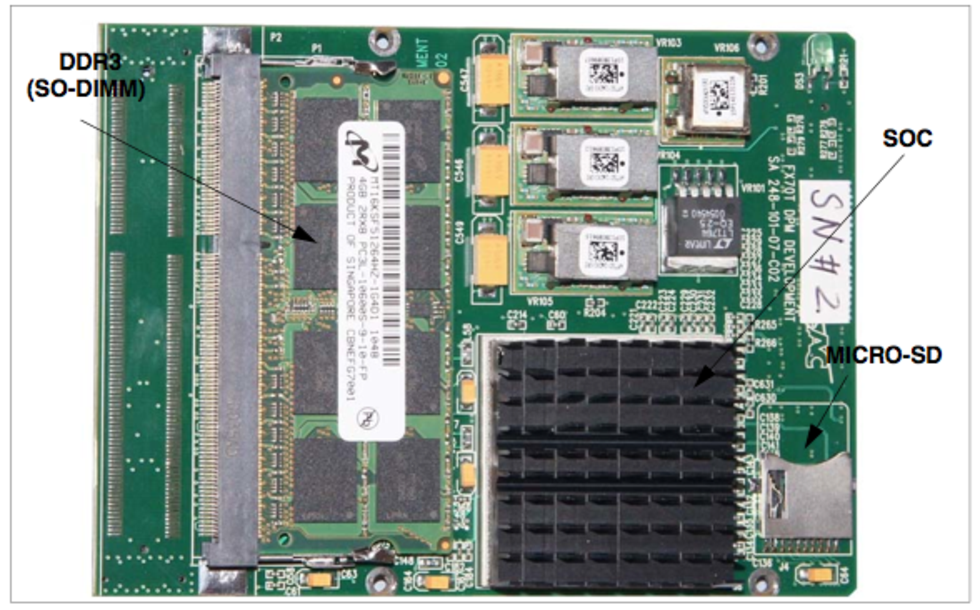
\includegraphics[scale=0.8]{mezzanine.pdf}
\caption{A single element RCE on a mezzanine board.}
\label{fig:mezz}
\end{figure} 


\subsubsection{Pretty Good Protocol}
\label{sec:PGP}
The Pretty Good Protocol (PGP) is a VHDL module which facilitates the bi-directional transmission of frame based messages over a two-wire physical link.      